\documentclass{usmthesis}
%%%%%%%%%%%%%%%%%%%%%
%These are all "libraries" or packages. You can include new ones here.
%%%%%%%%%%%%%%%%%%%%%
\usepackage{marvosym}
\usepackage{enumitem}
\usepackage{listings}
\lstset{basicstyle=\ttfamily,breaklines=true}
\usepackage{algorithm}
\usepackage{algorithmic}
\usepackage{indentfirst}
\usepackage{afterpage}
\usepackage{amssymb}
\usepackage{varwidth}
\usepackage{array}
\usepackage{pdflscape}
\usepackage{amsthm}
\usepackage{enumitem}
\newtheorem{myDef}{Definition}
\newtheorem{myLem}{Lemma}
\usepackage{tocloft}
\usepackage{tikz}
\usetikzlibrary{perspective}
\newcolumntype{M}[1]{>{\begin{varwidth}[t]{#1}}l<{\end{varwidth}}}
	
%%%%%%%%%%%%%%%%%%%%%
%Update your information here
%%%%%%%%%%%%%%%%%%%%%
\author{LI YU}	
\title{Boomerang Attacks on KATAN Revisited}
\titlems{Serangan Boomerang ke atas KATAN Dilawati Semula}
\submityear{2022}
\submitmonth{January}
%Doctor of Philosophy/Master of Science
\degreetype{Master of Science}

%Don't edit the following%
\newcites{own}{List of Publications}

\ifpdf
  \makeatletter
  \usepackage[pdftex,plainpages=false,hypertexnames=false,bookmarksnumbered,pdfpagelabels,%
    pdfauthor={\@author},pdftitle={\@title}]{hyperref}
  \makeatother
\else
  \usepackage[dvips,plainpages=false,bookmarksnumbered,breaklinks=true]{hyperref}
\fi

\usepackage{ragged2e}

\begin{document}

\bibliographystyle{apacite}
\bibliographystyleown{apacite}
\frontmatter
\frontmatter
\makecover

%Edit files in FrontMatter folder
\chapter{Declaration}
\thispagestyle{empty}
\noindent Name: LI YU \\
Matric No: P-COM0067/21 \\
School: School of Computer Sciences \\
Thesis Title: Boomerang Attacks on KATAN Revisited \\

\noindent I hereby declare that this thesis I have submitted to ........................................................ on ......................................... is my own work. I have stated all references used for the completion of my thesis.\\
\noindent I agree to prepare electronic copies of the said thesis to the external examiner or internal examiner for the determination of amount of words used or to check on plagiarism should a request be made.\\
\noindent I make this declaration with the believe that what is stated in this declaration is true and the thesis as forwarded is free from plagiarism as provided under Rule 6 of the Universities and University Colleges (Amendment) Act 2008, University Science Malaysia Rules (Student Discipline) 1999.\\
\noindent I conscientiously believe and agree that the University can take disciplinary actions against me under Rule 48 of the Act should my thesis be found to be the work or ideas of other persons.\\


\noindent Students Signature: .................................................. Date: ........................................\\
\noindent Acknowledgement of receipt by: ............................. Date: ........................................
\chapter{Acknowledgement}

This thesis would not have been a success without ......


\begin{singlespace}
\tableofcontents \clearpage
\listoftables \clearpage
\listoffigures \clearpage

%%%%%%%%%%%%%%%%%%%%%%%%%%%%%%%%%%%%%%%%%%%%%%%%%%%%%%%
% You can comment out the following line if you don't
% have a "List of Plates"
%%%%%%%%%%%%%%%%%%%%%%%%%%%%%%%%%%%%%%%%%%%%%%%%%%%%%%%
%\listofplates \clearpage

%%%%%%%%%%%%%%%%%%%%%%%%%%%%%%%%%%%%%%%%%%%%%%%%%%%%%%%
% You can comment out the following line if you don't
% have a "List of Acronyms"
%%%%%%%%%%%%%%%%%%%%%%%%%%%%%%%%%%%%%%%%%%%%%%%%%%%%%%%
\chapter{List of Abbreviations}
\begin{acronym}[NESSIE] %% replace 'MMMM' with the longest acronym in your list
\acro{3DES}{Triple Data Encryption Standard}
\acro{3GPP}{3rd Generation Partnership Project}
\acro{AE}{Authenticated Encryption}
\acro{AEAD}{Authenticated Encryption with Associated Data}
\acro{AES}{Advanced Encryption Standard}
\acro{ARX}{Addition Rotation Xor}
\acro{AS}{Active S-box}
\acro{ASE}{Average Shannon Entropy}
\acro{CBC}{Cipher Block Chaining}
\acro{CCML}{Coupled Chaotic Map Lattice}
\acro{CFB}{Cipher Feedback}
\acro{CPU}{Central Processing Unit}
\acro{CTR}{Counter}
\acro{DES}{Data Encryption Standard}
\acro{DDR}{Data-Dependent Rotation}
\acro{ECB}{Electronic Codebook}
\acro{FFT}{Fast Fourier Transform}
\acro{FIPS}{Federal Information Processing}
\acro{FxP}{Fixed Point} 
\acro{FSM}{Finite State Machine}
\acro{GCC}{GNU Compiler Collection}
\acro{GCM}{Galois Counter Mode}
\acro{GFS}{Generalized Feistel Structure}
\acro{GK}{Generator Kernel}
\acro{GOP}{Gray Ordering Number}
\acro{GPU}{Graphics Processing Unit}
\acro{GSM}{Global System for Mobile Communications}
\acro{HDD}{Hard Disk Drive}
\acro{IEC}{International Electrotechnical Commission}
\acro{ISO}{International Organization for Standardization}
\acro{IV}{Initialization Vector}
\acro{KFB}{Key Feedback}
\acro{LCG}{Linear Congruential Generator}
\acro{LCM}{Least Common Multiple}
\acro{LFSR}{Linear Feedback Shift Register}
\acro{LSB}{Least Significant Bit}
\acro{MAC}{Message Authentication Code}
\acro{Mbps}{Megabits Per Second}
\acro{MDS}{Maximum Distance Separable}
\acro{MitM}{Meet-in-the-Middle}
\acro{MSB}{Most Significant Bit}
\acro{MLD}{Maximum-Likelihood Decoding}
\acro{MQ}{Multivariate Equation}
\acro{NESSIE}{New European Schemes for Signatures, Integrity and Encryption}
\acro{NIST}{National Institute of Standards and Technology}
\acro{NLF}{Nonlinear Filter}
\end{acronym}


\chapter{List of Symbols}
\begin{acronym}[]
\acro{length}[$|x|$]{Bit length of $x$.}
\acro{xor}[$\oplus$]{Bitwise XOR.}
\acro{and}[$\wedge$]{Bitwise AND.}
\acro{concat}[$x||y$]{Bitwise concatenation of $x$ and $y$.}
\acro{add}[$\boxplus$]{Modular addition.}
\acro{shift}[$(x<<y)$ / $(x>>y)$]{Bitwise left/right shift of $x$ by $y$ bits.}
\acro{floor}[$\lfloor x \rfloor$]{Floor function to map a real number $x$ to the previous largest integer.}
\end{acronym}

\end{singlespace}

% Paragraph spacing
\setlength\parskip{18pt}
% Text-float spacing
\setlength\intextsep{24pt}

%%%%%%%%%%%%%%%%%%%%%%%%%%%%%%%%%%%%%%%%%%%%%%%%%%%%%%%
% Your Malay and English abstracts, each in one file.
%%%%%%%%%%%%%%%%%%%%%%%%%%%%%%%%%%%%%%%%%%%%%%%%%%%%%%%
\begin{doublespace}
\begin{MsAbstract}

Abstrak Bahasa Malaysia ditulis di sini.
\end{MsAbstract}
\begin{EnAbstract}

English abstract here.

\end{EnAbstract}

\mainmatter

%Edit the main files. All your diagrams should be in the main folder, not the chapter folder
\chapter{Introduction}\label{chap:intro}
\section{Background}
The boomerang attack is currently the most popular cryptanalysis method, it is based on the differential method, and was proposed by \cite{10.1007/3-540-48519-8_12}. It is a chosen plaintext attack and is used to analysis symmetric cryptography, compare to differential cryptanalysis, which provides a more efficient method to analyse more complex ciphers. Here is a brief introduction to the principle. Figure \ref{fig:boomerang} shows the design of basic boomerang analysis.  The boomerang attack attempts to generate a quartet structure at an intermediate value halfway through the cipher. 

\begin{figure}[hbt!]
    \centering
    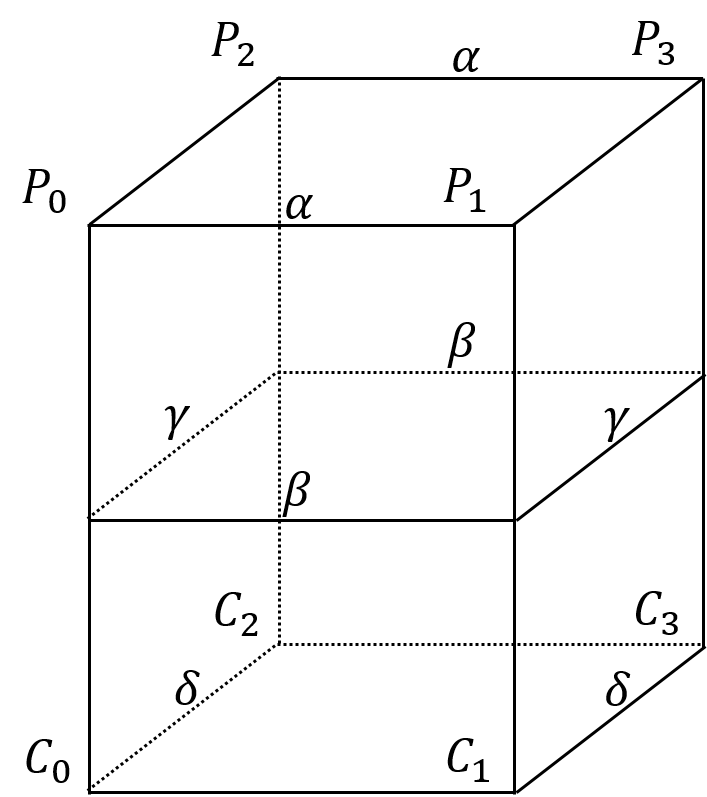
\includegraphics[width=45mm]{boomerang}
    \caption[Boomerang Attack Model]{Boomerang Attack Model}\label{fig:boomerang}
\end{figure}

The boomerang attack is widely used due to its power. However, \cite{5730575} raised concerns about the validity of the boomerang attack results that not all S-BOX ciphers boomerang distinguishers are reliable, for S-BOX based ciphers, two independently chosen differential trails can be incompatible, thus the probability of finding a right quartet can be zero and the same phenomenon was observed by \cite{10.1007/978-3-540-45146-4_12} as the middle round S-box trick. In order to solve this problem, \cite{10.1007/978-3-319-78375-8_22} proposed a new cryptanalysis tool called Boomerang Connectivity Table (BTC). Compared to the Difference Distributed Table (DDT), BTC can find better differential trails, the table [1] from the paper demonstrates the advantage. BTC has better efficiency than DDT, but it has only been used in practice on the S-BOX cipher so far, \cite{10.1007/978-3-319-78375-8_22} point out BTC may also be valid for modular addition ciphers.

With the development of IoT, more and more low-end devices are used, such as Smart Locks, there are large holdings of these devices, leading to an increasing need to provide security. Because these devices have the low computing power and run in a complex environment, several lightweight block ciphers were proposed. The KATAN family is based on modular addition, not S-BOX and was proposed by \cite{10.1007/978-3-642-04138-9_20}. Although it is subjected to many different types of analysis, it still provides security. The KATAN family contains six ciphers divide into two flavors, and all block ciphers share the 80-bits key size. KATAN is composed of three block ciphers, with 32,48, or 64-bits block size.  \cite{inproceedings} use an extended boomerang framework in related-key setting, to achieve the best results by far for KATAN48/64 in differential setting.




\section{Problem Statement}
As described in the previous section, the cryptanalysis based on boomerang has achieved good results \cite{inproceedings} on the KATAN cipher so far, but as \cite{5730575} point out, distinguishers based on boomerang analysis are not necessarily reliable. In other words, BTC \cite{10.1007/978-3-319-78375-8_22} can achieve a better result on S-BOX ciphers. So, there are some questions that need to be discovered:
\begin{enumerate}
    \item Whether BTC can apply non-S-BOX ciphers?
    \item How to improve the reliability of the result of the boomerang analysis of KATAN?
\end{enumerate}
Then, the following research questions will be answered in this work:
\begin{enumerate}
    \item What strategies can make BTC apply to ciphers based on modular operation, such as KATAN?
    \item How can achieve better results of boomerang analysis of KATAN than previous research using BTC?
\end{enumerate}


\section{Research Motivation}
With the rise of edge computing and the Internet of things, many devices need to save data locally, which also leads to high security for such devices. To improve the security of these devices without reducing performance, several lightweight cipers were proposed. KATAN is one example of them. It has withstood various cryptanalysis since it was proposed and still provides high security. This work uses it as a target cipher because it widely used in RFID devices, which represent a huge commercial value, and its analysis can further guarantee the security of the assets it protects. On the other hand, KATAN is a cipher based on modular addition, which can help this work to verify the adaptation of BTC on non-S-BOX ciphers. 

This work chose the boomerang attack as the cryptanalysis method because the efficiency of the boomerang attack was demonstrated in several research projects. This helped this work reduce the likelihood of failure, and due to the boomerang attack has become a research hotspot, many strategies which improve the efficiency of the attack were proposed. In conclusion, this work can achieve the better result by using the boomerang attack.

\section{Research Scope and Objectives}
\subsection{Research Scope}
This study consists of two parts. First, in cryptography, this work focus on block ciphers, which are symmetric-key cryptosystem.  Second, in cryptanalysis, this work focus on boomerang attack, which is an adaption of differential cryptanalysis. In short, the scope of this study is that boomerang attack on non-S-BOX block ciphers.

\subsection{Research Objectives}
According to this study research questions, the objectives of this research are summarized as follows:
\begin{enumerate}[noitemsep]
\item BTC be successfully applied on KATAN ciphers.
\item To improve the result of boomerang attack on KATAN ciphers by using BTC.
\end{enumerate}
Two objectives should be enough, and each objective should be measurable.

\section{Research Methodology}
This study has six steps, are shown in Figure \ref{fig:method}.
\begin{figure}[hbt!]
\centering
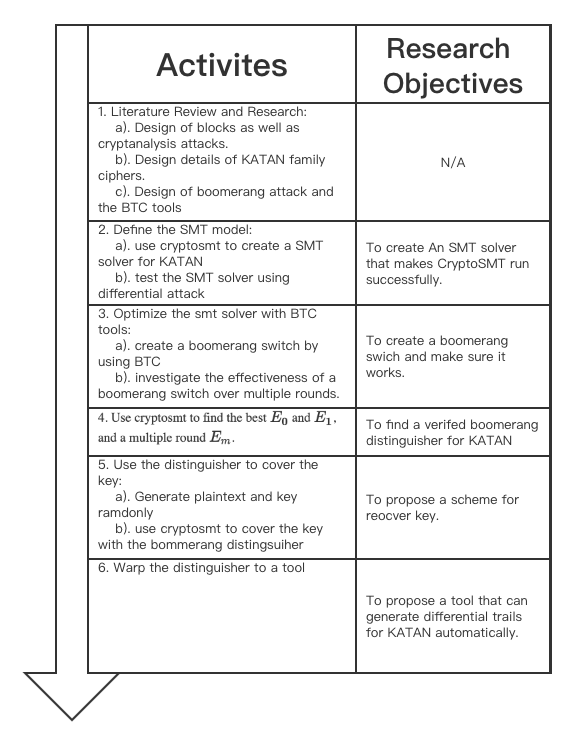
\includegraphics[width=150mm]{rm.png}
\caption[Research Framework]{Research Framework}\label{fig:method}
\end{figure}

\section{Research Contributions}


This study gets some contributions to cryptanalysis.

First, \cite{10.1007/978-3-319-78375-8_22} point out the BTC tools may be applied on ciphers based on modular addition operation, but it is not practiced. This study successfully demonstrates the BTC tools are not only used on ciphers based on S-BOX and useful to ciphers based on modular addition operations. The contribution can help cryptanalysts to improve their distinguisher of attack to ciphers based on modular operations.

This work also improves the probability of the boomerang distinguisher of KATAN. For KATAN48/64, this work was able to greatly improve upon the previous results to achieve the best result by for. The rules reflected in this distinguisher can help designers design ciphers better.

Last, this work proposed a tool that can generate distinguishers automatically, which can help improve the efficiency of attacking KATAN. Then summarize the contributions of this work as follows:

\begin{itemize}
\item A new strategy that can use BTC on ciphers based on modular addition operation.
\item Improve the probability of the distinguisher for KATAN.
\item A new cryptanalysis tool that can generate distinguishers for KATAN automatically.
\end{itemize}

\section{Thesis Outline}
Chapter 1 has provided an overview of the research including the introduction for KATAN and boomerang attack, and what is this study going to solve.

Next, Chapter 2 provides an in-depth review of prior work in the fields including block ciphers, KATAN, differential attack, boomerang attack and BTC.

Chapter 3 discusses the methodology involved in this research, we demonstrate the boomerang distinguisher search and key recovery attack on the KATAN family by using BTC. This is followed by Chapter 4 which analyses the findings and results, the BTC tools improve the probability of finding the right quartet.

Finally, this thesis concludes in Chapter 6 with a summary of finding and future works.
 %Contains a sample image
\chapter{Literature Review}\label{chap:review}
\section{Overview}
The research analyzes previous cryptanalysis work, including the design of block ciphers, cryptanalysis-related knowledge, including KATAN and Boomerang related literature needed for the research.


\section{Block ciphers and Cryptanalysis}\label{sec:symmetric_review}
This section describes the principle of symmetric-key encryption and introduces two symmetric-key ciphers. Then there is a review of cryptanalysis methods, and the details of these methods are described. This section provides help for understanding cryptanalysis.

\subsection{Block Cipher Designs}

Block cipher is an important part of symmetric-key encryption. The design concept of block cipher originated from \cite{6769090}. Its public research began with the publication of the DES algorithm \cite{pub1999data} in the late 1970s. The rapid development of block cipher theory and application Benefited from the AES \cite{dworkin2001advanced} program in the United States in the late 1990s  and the NESSIE program in Europe in the early 2000s. 

In the literature \cite{6769090}, from the perspective of resisting statistical attacks, Shannon proposed the ”confusion” and ”diffusion” criteria for designing encryption algorithms. Each element in the original text is rearranged in obfuscation, whereas in diffusion, each element is changed to be mapped to numerous elements in the ciphertext. This criterion is still one of the important principles to be followed in the design of block ciphers. In the AES plan and the NESSIE plan, the cryptography community has conducted extensive and in-depth research on the design and analysis theory of block ciphers, and the theory of block ciphers is perfect. In the SHA-3 project \cite{dworkin2015sha}, more than half of the Hash functions adopt the design concept of block ciphers, so block ciphers are becoming more and more important. 

The design of block ciphers usually follows the following two principles: the security principle and the implementation principle. The security principles include the principle of confusion, the principle of proliferation, and the principle of resistance to existing attacks. Implementation principles include software implementation principles and hardware implementation principles. Usually, the designed algorithm conforms to the above principles by iterative means: one method is to construct an iterative function with strong cryptographic properties, so that the number of iterations can be reduced; the other method is to construct an iterative function with relatively weak cryptographic properties, but The number of iterations is relatively high. In practical construction, the latter is usually adopted, that is, functions with weak cryptographic properties are iterated for many times to satisfy the security principle and the realization principle. 

The mathematic model of block cipher, $\mathbb{F}_2$ presents a binary field, $\mathbb{F}_2^n$ and $\mathbb{F}_2^m$ present $n$ and $m$ dimensional vector spaces, respectively. $S_K\in \mathbb{F}_2^m$ is a key space, then the ciphers can present two reflections.

\begin{equation}
    \begin{aligned}
        E: F_2^n \times S_k \to F_2^n,\\
        D: F_2^n \times S_k \to F_2^n.
    \end{aligned}
\end{equation}


The basic structure of commonly used block ciphers will be described below.

\subsubsection{Feistel Structure}
The IBM researchers that developed the DES algorithm also came up with the Feistel structure, which eventually gained popularity. Referring to Figure \ref{fig:Feistel}, the encryption procedure for the r-round Feistel structure cipher with a $2n$ block length is as follows: Given a civilization $P$ with $2n$ bits, divide it into two left and right n bits, where $L_0$ is the left $n$ bits and $R_0$ is the right $n$ bits, and then, in accordance with \eqref{eq:Feistel}, repeat the procedure $r$ times.

\begin{equation}
    \begin{aligned}
        \begin{cases}
            L_i = R_{i-1}\\
            R_i=L_{i-1}\oplus F(R_{i-1},K_i)
        \end{cases}
    \end{aligned}  
    i=1,2,\dots,r  
    \label{eq:Feistel}
\end{equation}

Here, $\oplus$ denotes an XOR operation, $F: \mathbb{F}^n_2\times \mathbb{F}^m_2\to \mathbb{F}^n_2$ stands for "round," and $K_1,K_2,\dots, K_r$ According to the key expansion method, $K_r$ is the round key produced by the seed key $K$, and $m$ is the round key's length. The final round typically does not require "left and right exchange," meaning that the ciphertext is $C=R_rL_r$. The slower diffusion effect is a drawback of Feistel.


\begin{figure}[hbt!]
    \centering
    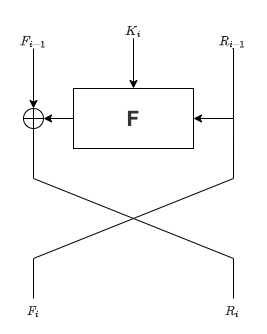
\includegraphics[width=45mm]{Feistel}
    \caption[Boomerang Attack Model]{Feistel Structure}\label{fig:Feistel}
\end{figure}

\subsubsection{SPN Structure}
A reversible linear transformation P and a reversible nonlinear function S, controlled by a round key, typically make up each round of the SPN structure. The S-transform layer serves as the obfuscation layer in this construction, and the P-transform layer serves as the diffusion layer. The SPN structure has a faster diffusion effect than the Feistel structure, and the designer can use this structure to provide algorithms resistant to differential cryptanalysis and linear ciphers with a provable security for analysis.
\begin{equation}
    \begin{aligned}
        \begin{cases}
            Y&=S(X_{i-1},K_i)\\
            X_i&=P(Y)
        \end{cases}
    \end{aligned}
    i=1,2,\dots,r  
    \label{eq2}
\end{equation}
The encryption procedure for the r-round SPN structure cipher with an n-block length is as follows: Let $P=X_0$, where $P$ is the plaintext with $n$ bits, and follow \eqref{eq2} to carry out the same procedure for $r$ rounds.

In SPN structured ciphers, the last round of $P$ transformation is usually replaced by key addition.

\begin{figure}[hbt!]
    \centering
    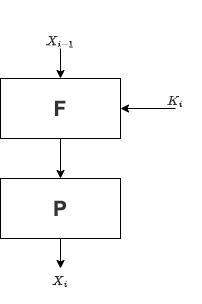
\includegraphics[width=45mm]{SPN}
    \caption[Boomerang Attack Model]{SPN Structure}\label{fig:SPN}
\end{figure}

\subsubsection{Lai-Massey Structure}
When developing the IDEA algorithm, Lai and Massey proposed a framework they called the Lai-Massey structure. Most of the time, the Lai-Massey structure has the benefit of consistent encryption and decryption.

\begin{figure}[hbt!]
    \centering
    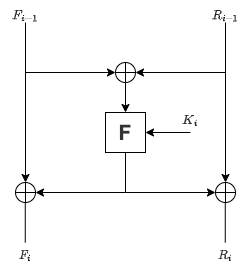
\includegraphics[width=45mm]{Lai_Massey.png}
    \caption[Boomerang Attack Model]{Lai-Massey Structure}\label{fig:Lai_Massey}
\end{figure}

For the r-round Lai-Massey structure cipher with a block length of 2n, the encryption process is as follows: Given a 2n-bit plaintext $P$, first divide it into two n-bit parts on the left and right, and denote $L_0$ as the left $n$ bits of $P$, and $R_0$ as the right $n$ bits of $P$, then $P=L_0R_0$. Then according to \eqref{eq3}, $r$ rounds of exactly the same operations are performed.

\begin{equation}
    \begin{aligned}
        \begin{cases}
            T&=F(L_{i-1}\oplus R_{i-1},K_i)\\
            L_i&=L_{i-1}\oplus T\\
            R_i&=R_{i-1}\oplus T
        \end{cases}
    \end{aligned}
    i=1,2,\dots,r  
    \label{eq3}
\end{equation}

\subsubsection{Summary}
The overall structure is an important feature of block cipher algorithms. Different structures have a great impact on the selection of the round function and the performance on various platforms. In addition to the above three mainstream structures, the overall structure also includes generalized (non-)equilibrium Feistel structure, MISTY structure and the mixed use of various structures. In addition, the round functions of many cryptographic algorithms adopt different structures. For example, the Camellia algorithm adopts the Feistel structure as a whole, but the round function adopts the SPN structure; the FOX algorithm adopts the Lai-Massey structure as a whole, and the round function adopts the SPS structure. The structure used to design an algorithm mainly depends on the performance requirements of the algorithm, the construction of sub-modules, and the security of the overall structure.


\subsection{KATAN family cipher}
KATAN family cipher is a hardware oriented block ciphers and was proposed in CHES 2009 \cite{10.1007/978-3-642-04138-9_20}. KATAN family has three variants of KATAN are KATAN32, KATAN48 and KATAN64. Each various contains six block ciphers divide into two flavors, in the first flavor is composed of three block ciphers, with 32,48 or 64 bit block size, and in the second flavor contains the other three ciphers with same block size. They are use 80-bit key size. KATAN use an extending key algorithm to make 80-bit key to 508bit sub-key. Suppose a key $k$ is 80-bit, and $k_i$ present i-th bit in $K$, the sub-key is given by:
\begin{equation}
    sk_i=
\left\{
    \begin{aligned}
        &k_i\qquad\qquad\qquad for\quad i = 0\dots 79\\
        &k_{i-80}\oplus k_{i-61}\oplus k_{i-50}\oplus k_{i-13}\quad Otherwise
    \end{aligned}
\right.
\end{equation}The round function of KATAN, the plaintext be divided two part and be loaded to two register $L_1$ and $L_2$, then the update processes are shown as follows:
\begin{equation}
    \begin{aligned}
        f_a(L_1) &= L_1[x_1]\oplus L_1[x_2]\oplus (L_1[x_3])\cdot L_1[x_4])\oplus(L_1[x_5]\cdot IR)\oplus k_a\\
    f_b(L_2) &= L_2[y_1]\oplus L_2[y_2]\oplus (L_2[y_3])\cdot L_2[y_4])\oplus(L_2[y_5]\cdot L_2[y_6])\oplus k_b\\
    L_1[i] &= L_1[i-1](i\leq i\le |L_1|), L_1[0]=f_b(L_2),\\
    L_2[i]&=L_2[i-1](i\leq i\le |L_2|), L_2[0]=f_b(L_1),\\    
    \end{aligned}
\end{equation}
 where $\oplus$ and $\cdot$ are bitwise $XOR$ and $AND$ operations, respectively, and $L[x]$ denotes the x\-th bit of $L$, $IR$ is the round constant value defined in the specification, and ka and kb are two subkey bits. For round $i$, $k_a$ and $k_b$ correspond to $sk_{2(i-1)}$ and $sk_{2(i-1)+1}$. The parameters of KATAN family are shown in TABLE \ref{tb:KATAN_P}.
 \begin{table}[htbp]
	\centering  
	\caption{Parameters of KATAN family} 
	\label{tb:KATAN_P} 
	\begin{tabular}{|c||c|c|c|c|c|c|c|c|c|c|c|c|c|c|c|c|}  
        \hline  
        algorithm&|$L_1$|&|$L_2$|&$x_1$&$x_2$&$x_3$&$x_4$&$x_5$&$y_1$&$y_2$&$y_3$&$y_4$&$y_5$&$y_6$\\
		\hline  
		KATAN32&13&19&12&7&8&5&3&18&7&12&10&8&3\\
        KATAN48&19&29&18&12&15&7&6&28&19&21&13&15&6\\
        KATAN64&25&39&24&15&20&11&9&38&25&33&21&14&9\\
		\hline
	\end{tabular}
\end{table}






\subsection{Cryptanalysis}
There are two basic ways to measure the security of a cryptographic algorithm: one is actual security, and the other is unconditional security (theoretical security). The actual security is evaluated according to the amount of computation required to decipher the cryptosystem. For example, the security of the RSA system is based on the difficulty of decomposing large integers, but with the development of computer technology, RSA may also be vulnerable. Theoretical security is independent of an adversary's computing power and time, and any effort to decipher an algorithm will be no better than random selection. 

Most of the cryptanalysis methods proposed in the papers follow Kerckhoffs's principle: The principle holds that a cryptosystem should be secure, even if everything about the system, except the key, is public knowledge. According to the Kerckhoffs's principle, the security of a cryptographic algorithm should depend on the secrecy of the key, not the secrecy of the algorithm itself.

Many literatures propose different cryptanalysis methods to analyze the target algorithms they specify. What is important is whether these algorithms have extremely high accuracy, whether they undermine practical security or theoretical security, in which threats to practical security are very serious issues. In the following, we provide an overview of the cryptanalysis of block ciphers.

The method of cryptanalysis is divided into brute force attack, the security of the algorithm is studied based on the mathematical method, and the security of the algorithm and the security of the algorithm under different usage modes are studied in combination with the physical realization method. 

According to the different environments, password attacks can be divided into the following four types:
\begin{itemize}
    \item Ciphertext-only attack: A cryptanalyst has one or more ciphertexts encrypted with the same key, and analyzes these decrypted ciphertexts to obtain the plaintext or key.
    \item Known-Plaintext Attack: A cryptanalyst has some plaintexts and ciphertexts of these plaintexts encrypted with the same key, and recovers the key by analyzing these known plaintexts and the corresponding ciphertexts.
    \item Chosen-plaintext attack: The cryptanalyst can choose the plaintext he wants at will and encrypt it, and recover the key according to the selected plaintext and the corresponding ciphertext.
    \item Chosen ciphertext attack: The cryptanalyst can freely select the ciphertext he wants and decrypt it, and recover the key according to the chosen ciphertext and the corresponding plaintext.
\end{itemize}Then, the research on analytical ciphers is usually based on three different foundations.

\subsubsection{Brute-force}
Brute-force attacks are the simplest and least effective, they generally include four methods:\begin{itemize}
    \item Exhaustive key search: Under a ciphertext-only attack, the attacker uses all possible keys to continue decrypting one or more ciphertexts until a meaningful plaintext is obtained. This method can decipher any block cipher in theory, but its efficiency is the lowest. In practical cryptanalysis, it is usually used in combination with other analysis methods.
    \item Dictionary attack: The attacker collects pairs of plaintext and ciphertext and arranges them into a "dictionary". When seeing a ciphertext, the attacker checks whether it exists in the dictionary, and if so, finds the corresponding plaintext.
    \item Table lookup attack: This method is a chosen plaintext attack. The attacker uses all possible keys to encrypt the same plaintext, and stores the key and the corresponding ciphertext. When obtaining the plaintext and ciphertext, the attacker only needs to Find the corresponding key in the storage table.
    \item Time-tradeoff attack: This is a chosen-plaintext attack method, proposed by Hellmma, by using a combination of exhaustive key search and table lookup attack.
\end{itemize}Although these methods are not very useful in practice, the complexity of exhaustive key search is used as an indicator to measure the efficiency of an attacking algorithm. 

\subsubsection{Based on the Security of Algorithms Based on Mathematical Methods}
This method mainly includes two aspects: one is to study how to distinguish cryptographic algorithms from random permutation. In cryptanalysis, for the same indicator, first calculate its value under random permutation, and then calculate the corresponding value of a cryptographic algorithm in a certain cryptographic algorithm. If the two values are significantly different, then this metric can distinguish a cryptographic algorithm from random permutation. In cryptanalysis, if for some specific form of plaintext input, the corresponding ciphertext follows a special rule, it is said to find an effective distinguisher of the algorithm. The second is to study how to obtain the key information of the cryptographic algorithm. For iterative block ciphers, the cryptanalyst first finds an efficient distinguisher of the reduced-rounds algorithm, and then verifies the correctness of the distinguisher by guessing some of the round keys. When an effective distinguisher of the cryptographic algorithm is found, there are usually two ways to recover the secret: one is the statistical method, for the guess value of each key, according to certain rules (usually related to the distinguisher) collected plain ciphertext Statistical analysis is performed, and the final value with a clear statistical advantage may be the correct key. The another is to solve by algebraic method. In this method, the transformation corresponding to encryption and decryption is represented by a system of equations. Through certain mathematical methods, the root of the system of equations is solved to obtain the key information. Common math-based methods include:
\begin{itemize}
    \item differential cryptanalysis
    \item linear cryptanalysis
    \item meet-in-the-middle attack
    \item collision attack 
    \item Square attack 
    \item interpolation attack
    \item correlated key attack 
    \item boomerang attack
\end{itemize}
With the development of cryptanalysis, more methods have been proposed.

\subsubsection{The security of algorithms is related to they way it is implemented in hardware}
In the traditional research on the security of algorithms based on mathematical methods, the encryption or decryption process of the algorithm is generally regarded as a transformation with secret parameters, and the key information is inferred only by obtaining the input and output of the transformation. At the end of the 20th century, a new attack method appeared in the cryptography world. In addition to the traditional mathematical method, this attack method also combines the information differences represented by certain physical parameters such as time, energy, electromagnetic, temperature, sound, etc. to infer information about the key. This attack method combined with physical implementation is generally called side channel attack. At present, common side-channel attacks mainly include timing attacks, energy analysis, fault attacks, electromagnetic attacks, and cache attacks.

\section{Cryptanalysis Method}\label{cry_method}
This section describes details of several attacks.

\subsection{Differential Attack}
The differential attack is one most effective methods to attack iterative block ciphers,  and it is an important index for evaluating the security of block ciphers. \cite{biham1991differential} proposed this analysis method. It finds the difference between specific pairs of plaintext and ciphertext to distinguish block ciphers from random permutations and then recovers the key. 

We assume a block cipher, $E\{0,1\}^n \times \{0,1\}^l \to \{0,1\}^n$, and $n, l$ present length of a block and length of the key, respectively. For $k \in \{0,1\}^l$, the permutation be presented $E_k(\cdot)=E(\cdot, k)$ on $\{0,1\}^n$. The encryption function $E_k(\cdot)$ is consist of $r$ sub\-encryption functions which use sub-key $k_i, i=1,2,3,4…,r$ to encrypt. The encyrption equation as \ref{block_cipher_eq}.

\begin{equation}
    \label{block_cipher_eq}
    E_k(x)=F_{k_r}\circ F_{k_{r-1}}\circ \dots \circ F_{k_2}\circ F_{k_1}(x).
\end{equation}
Next, $Y_{i-1}, Y_i$ present the input and output on i-th round, in other words, $Y_i=F_{k_i}(Y_{i-1})$. $X,Z=Y_r$ present the input(plaintext) of the first round and the output of the last round, respectively. There are three important definitions. First, \textbf{Difference}, the difference of $X, X^*\in\{0,1\}^n$ is $\Delta X = X\oplus X^*$. Second, \textbf{Differential}, presents a propagation from difference $\alpha$ to difference $\beta$.
Last, \textbf{Differential characteristic}, a differential characteristic of $i$ rounds, $\Omega = (\beta_0,\beta_1\dots,\beta_{i-1},\beta_i)$ when the difference of the input pairs $(X,X^*)$ satisfy $X\oplus X^*=\beta_0$, and in i-th round, the middle states $(Y_j ,Y_j^*)$ satisfy $Y_j\oplus Y_j^*=\beta_j$. The equation \ref{eq:DP_alpha_beta} presents the probability of a differential,
\begin{equation}
    \label{eq:DP_alpha_beta}
DP(\alpha,\beta) = \underset{X,K}{Prob}\{F(X,K)\oplus F(X\oplus \alpha, K)=\beta\},
\end{equation} when the number of rounds more than 1 can derive the probability of a differential characteristic $\Omega = (\beta_0, \beta_1,\dots,\beta_i)$ in following.
\begin{equation}
DP(\Omega)=\prod_{j=1}^iDP(\beta_{j-1}, \beta_j).
\end{equation}
In Feistel or SPN structure ciphers, the S-box is the only nonlinear part of the round function, so we need to make \textbf{Differential Distributed Table(DDT)} if we want to find a differential path with high probability. There is an example of DDT of present cipher is Figure \ref{fig:ddt}. The first row present difference of out, and first column present difference of input to S-BOX. Suppose $S:\{0,1\}^n\to\{0,1\}^n$ an n-bit to n-bit S-BOX,the element of DDT is given by:
\begin{equation}
    (\Delta_{in}, \Delta_{out})=\#\{P_i\oplus P_i^*=\Delta_{in}|S(P_i)\oplus S(P_i^*)=\Delta_{out}\}
\end{equation}
\begin{figure}[hbt!]
    \centering
    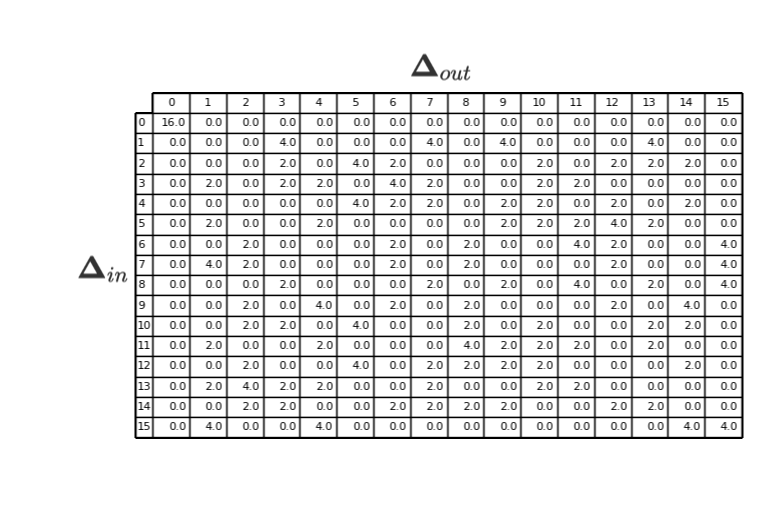
\includegraphics[width=100mm]{DDT.png}
    \caption[Differential Distributed Table]{Differential Distributed Table}\label{fig:ddt}
\end{figure}
The probability of a pair($\Delta_{in}, \Delta_{out}$) is $p=\frac{pos(\Delta_{in}, \Delta_{out})}{2^n}$. The differential attack steps are summarized as follows:
\begin{enumerate}
    \item To find a high probability differential characteristic of $r-1$ rounds, the probability is presented as $p$.
    \item To determine the sub-key in the i-th round by the output of the differential characteristic. Assume the length of the key attacked is $l$ bits, to set $2^l$ counters, each counter corresponding to each possible candidate key.
    \item Generate the plaintext  $X$ uniformly at random, $X^*$ satisfy $X^*=X\oplus \alpha$. To encrypt $X, X^*$ to get ciphertexts $Z, Z^*$, respectively. The number of generated plaintext pairs is $m \approx c \times \frac{1}{p}$, $c$ presents a constant number.
    \item For each ciphertext pairs, use candidate sub-key to decrypt $Z, Z^*$, the difference of the decrypted data $\Delta = F^{-1}_{gk_i}\oplus F^{-1}_{gk_i}(Z^*)$, if $\Delta = \beta$, then the counter corresponding to the candidate key is plus 1.
    \item The max value of these counter corresponding to the candidate key is correct sub-key.
\end{enumerate}

\subsection{Linear Cryptanalysis}
A Japanese researcher \cite{matsui1993linear} proposed a new cryptanalysis method in Eurocrypt 1993. The same year, in Crypto 1993, he published new two linear approximation relations, and he use these relations to crack DES, using 12 workshops and 50 days. There are results of the first experimental analysis of DES in the open literature. Unlike differential cryptanalysis, linear cryptanalysis is a known-plaintext attack method. It distinguishes block ciphers and random permutations by finding effective linear approximation relations between plaintext and ciphertext and recovers the key. Remember a block cipher defined in \ref{block_cipher_eq}. In linear cryptanalysis, assume $a,b\in \{0,1\}^n$ and $a=(a_1,a_2,a_3,…,a_n), b=(b_1,b_2,…,b_n)$, $F(x,k)$ presents the round function,  given two linear mask $(\alpha,\beta)$, the linear expression approximation formula is
\begin{equation}
\alpha \cdot x \oplus \beta \cdot F(x,k).
\end{equation} 
In this formula, $\cdot$ present multiplication in a binary field. Assume $p$ presents the probability of the linear expression approximation formula of $\alpha$ and $\beta$, then the linear probability can present these:
\begin{equation}
\begin{aligned}
Bias: \zeta_F &= p(\alpha,\beta) - \frac{1}{2},\\
Correlation: Cor_F &= 2p(\alpha, \beta) -1,\\
Potential: Pot_F &= (p(\alpha, \beta)-\frac{1}{2})^2.
\end{aligned}
\end{equation}. In paper [28,39], if the define the linear expression approximation formula of  linear mask $(\alpha,\beta)$ is
\begin{equation}
LP(\alpha,\beta) = (2\cdot \underset{X,K}{Prob}\{\alpha \cdot X=\beta \cdot F(X,K)\}-1)^2
\end{equation}, the $LP$ can corresponding to $DP$ of differential cryptanalysis. The steps of linear cryptanalysis as follows:
\begin{enumerate}
    \item To find r-1 rounds differential approximation formula that bias $zeta(\alpha, \beta)$ relatively large.
    \item To determine the sub-key in the i-th round by the output of the differential characteristic. Assume the length of the key attacked is $l$ bits, to set $2^l$ counters, each counter corresponding to each possible candidate key.
    \item Select the plaintext $X$ uniformly at random. To encrypt $X$ to get ciphertext $Z$, respectively. The number of generated plaintext pairs is $m \approx c \times \frac{1}{\zeta^2}$, $c$ presents a constant number.
    \item For each ciphertext $Z$, decrypt it to get $Y_{r-1}$ using candidate sub-keys, if $\alpha x\cdot X\oplus \beta \cdot Y_{r-1}=0$, then the corresponding counter is plus 1.
    \item The max value of $|\frac{\lambda^i}{m}-\frac{1}{2}|$ of these counter corresponding to the candidate key is correct sub-key.
\end{enumerate}

\subsection{Boomerang Attack}
The boomerang attack is a differential-style attack, it can find a higher probability of differential characteristics than a differential attack and it is a more effective cryptanalysis method of block ciphers. \cite{10.1007/3-540-48519-8_12} proposed this attack upon discovering good differential characteristics for the first four and last four Feistel rounds of COCONUT98. The boomerang attack has more power when it combined with other cryptanalysis method, it has been demonstrated when it is used to break the full-round AES-192/256 \cite{biryukov2009related} and the full-round KASUMI \cite{biham2005related} in the related-key setting.


Figure \ref{fig:boomerang} shows the structure of the boomerang attack. Four plaintexts $P_1$, $P_2$, $P_3$, $P_4$ and with their respective ciphertexts $C_0$, $C_1$, $C_2$, $C_3$; The $E(\cdot)$ present the encryption operation and decompose the cipher into $E=E_0 \circ E_1$ where $E_0$ represent the first half of the cipher and $E_1$ presents last half. There are four differential trails, $\alpha\to \beta$ for $E_0$; $r\to\delta$ for $E_1$; $\delta \to r$ for $E_1^{-1}$ and $\beta\to\alpha$ for $E_0^{-1}$.

The pair $P_0$ and $P_1$ with the trail for $E_0$ and the pairs $P_0,P_2$ and $P_1,P_3$ satisfy the trails for $E_1^{-1}$, then the pair $P_2$, $P_3$ is set up to use the trail $\beta\to\alpha$ for $E_0^{-1}$. Consider the intermediate value after half of the rounds, when the previous three trails hold, the formula \ref{boomerang_1} tell why.

\begin{equation}
    \begin{aligned}
        \label{boomerang_1}
        E_0(P_2)\oplus E_0(P_3)&=E_0(P_0)\oplus E_0(P_1)\oplus E_0(P_0)\oplus E_0(P_2) \oplus E_0(P_1) \oplus E_0(P_3)\\
        &=E_0(P)\oplus E_0(P_1)\oplus E_1^{-1}(C_0)\oplus E_1^{-1}(C_2)\oplus E_1^{-1}(C_1)\oplus E_1^{-1}(C_3)\\
        &=\beta \oplus r \oplus r\\
        &=\beta
    \end{aligned}
\end{equation}
Because the other three differential trails are holding, when the equation is satisfied, a pair of plaintexts $P_2,P_3$ has the same difference as found in original plaintexts. The idea of boomerang attack is to use such quartet of plaintext and of ciphertext to find key information, and use the information to recover key. In section 4 of \cite{10.1007/3-540-48519-8_12} states that probability of a quartet, assume $p_0$ is the probability of the differential trail $\alpha\to\beta$ for $E_0$ and $p_1$ is the probability of the differential trail $\delta\to r$ for $E_1$. Then the probability $p$ of a right quartet satisfy
\begin{equation}
    p\ge p_0^2p_1^2.
\end{equation}

The boomerang attack has some variants, such as amplified boomerang analysis \cite{kelsey2000amplified} and rectangle analysis \cite{biham2001rectangle}. In recent years, a new cryptanalysis method \cite{dunkelman2020retracing} based on this idea has been proposed, called the retracing boomerang attack , this new attack reduces the complexity of the boomerang method to analyse AES(5-ROUNDS) from $2^{24}$ to $2^{16.5}$. Also, the boomerang attack can achieve more efficiency with other cryptanalysis methods, such as the related-key method. In \cite{inproceedings}, the boomerang attack with a related-key setting achieves the best result for the boomerang to analyse KATAN48/64. But \cite{5730575} published results of several experiments, to demonstrate the boomerang analysis can commonly give highly inaccurate probability values and he shows the boomerang attack is used to analyse DES and AES on some parameters, then the boomerang never comes back.

For the problem, \cite{10.1007/978-3-319-78375-8_22} gives a solution. It proposed new tools to improve the reliability of the sandwich attack, called Boomerang Connectivity Table(BTC). The sandwich attack is a boomerang-style attack depicted in Fig \ref{fig:sandwich}, it defines $E=E_1\cdot E_m\cdot E_0$ where $E_m$ is a relatively short operation satisfying some differential propagation among four texts with probability $r$, then the entire probability is $p^2q^2r$. \cite{dunkelman2010practical} define r as follows.
\begin{equation}
    r=Pr[(x_3\oplus x_4)=\beta|(x_1\oplus x_2=\beta)\wedge (y_1\oplus y_3=r)\wedge(y_2\oplus y_4)=r]
    \label{r_prob}
\end{equation}
The BTC can evaluate $r$ in efficacy and easy-to-understand way when $E_m$ is composed of a single S-BOX layer. In this situation, for a given pair of ($\Delta_i, \bigtriangledown_o$), the probability that a right quartet is generated in each S-BOX in the middle S-BOX layer is given by:
\begin{equation}
\frac{\#\{x\in{0,1}^n|S^{-1}(S(x)\oplus \bigtriangledown_o)\oplus S^{-1}(S(x\oplus \Delta_i)\oplus \bigtriangledown_o)=\Delta_i\}}{2^n}
\label{btc_p}
\end{equation}
Where $S:\{0,1\}^n\to \{0,1\}^n$ is an n-bit to n-bit S-box and $S^{-1}$ is its inverse. When $E_m$ is a single S-BOX layer, the result of Equation\ref{btc_p} is exactly r in Equation\ref{r_prob}. \cite{10.1007/978-3-319-78375-8_22} demonstrate that the result of using BTC is more than the result only using DDT.
\begin{figure}[hbt!]
    \centering
    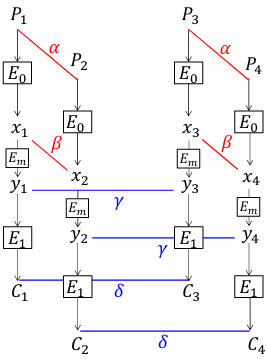
\includegraphics[width=45mm]{sandwich.png}
    \caption[Boomerang Attack Model]{Sandwich Attack Model}\label{fig:sandwich}
    \end{figure}

The BTC is not a panacea and can only use ciphers based on S-BOX in practice so far. There is discuss BTC use to ciphers based on ARX in \cite{10.1007/978-3-319-78375-8_22}, also points out S-BOX swich not work in ARX.

\section{Chapter Summary}\label{sec:lit_summary}

Section \ref{sec:symmetric_review} discussed the design of block ciphers and introduces three types of design structures, then introduces the basic theory of cryptanalysis and the design of KATAN. Section \ref{cry_method} describe the detail of the differential attack, the linear attack and boomerang attack, and discuss the advantages and disadvantages of BTC, this contents of this section are closely related to this study.
\chapter{Methodology}\label{chap:methodology}
\section{Overview}
This chapter describes all processes of this experiment. There are six steps, and each step has a corresponding goal. The steps are shown in Fig\ref{fig:method}. 


\section{Experiment}\label{sec:experiment}

\section{Literature Review and Research}
In this step, we reviewed the open literature, including block ciphers, KATAN, several attacks and BTC. We went through this step to explore whether BTC can make the results of Boomerang attack more credible, and determine how to improve BTC.

\section{Define the SMT model}
In this step, we analyze KATAN's cryptographic primitives, write Python code that can run on CryptoSMT, and then run differential analysis tests on CryptoSMT to ensure that the code is runnable. This step, we obtain a usable SMT model of KATAN.

\section{Optimize the smt solver with BTC tools}\label{m3}
In this step, we code the smt solver with BTC, and use data that be generated randomly to test and investigate the smt solver over multiple rounds, in the end, we get a boomerang switch.

\section{Find the best differential trails}\label{m4}
In this step, we use the boomerang switch that be created in \ref{m3}, to find the best $E_0$ and $E_1$ and a multiple round $E_m$. In the end, we can crate a verified boomerang distinguisher for KATAN.

\section{Cover the key}
In this step, we generate plaintext and a key randomly, and use the data to cover the key with the boomerang distinguisher that be created in \ref{m4}. In this end, we design a scheme for recover key and recover the key successfully.

\section{Proposed A tools}
Last, when we create a tool using Python that includes the distinguisher we proposed in \ref{m4}, it can automatically generate differential paths for KATAN.


\section{Chapter Summary}
This Chapter describes our experimental steps and our desired goals.
%Proposal ends here. But if you have anything partially designed, you can include chapter 4. For proposal also, you can include a brief conclusion.
\chapter{Results and Discussion}\label{chap:results}

\section{Overview}
Overview of the chapter.

\section{Example Section 1}\label{sec:example1}
This chapter will discuss what you have achieved.

\section{Example Section 2}\label{sec:example2}
Provide graphs, charts, tables and discuss your findings. Link them to achieving your objectives.

\section{Chapter Summary}
Summarise the chapter. Section \ref{sec:example1} discussed.... Section \ref{sec:example2} discussed...
\chapter{Conclusion and Future Work}\label{chap:conclusion}
Summarise your findings here.

\section{Limitations and Future Work}\label{sec:limit}
Discuss limitations and future work here.

\section{Closing Statements}\label{sec:closing}
Discuss if your objectives has been achieved and provide a table to summarise. Table \ref{tab:conc_findings} will have Section links that do not work. You need to edit and put your own information.

\afterpage{
\clearpage
\thispagestyle{empty}
\begin{landscape}
\begin{table}[!htbp]
\caption{Summary of Findings and Results}
\label{tab:conc_findings}
\begin{tabular}{M{5cm}p{6cm}M{5cm}p{7cm}}
\hline
\textbf{Research Questions} & \textbf{Research Objectives} & \textbf{Findings} & \textbf{Results} \\
\hline
How can symmetric-key ciphers be secured against statistical-based cryptanalysis? & To develop symmetric encryption encryption schemes that can seamlessly integrate true random numbers to resist statistical-based cryptanalysis.   & \textbf{Section~\ref{sec:aead_trns_scheme}}:\newline AEAD-based scheme \newline \textbf{Section~\ref{sec:stream_trns_scheme}}:\newline Stream cipher-based scheme & \textbf{Section~\ref{sec:block_cipher_resistance}}: \newline Theoretical evaluation of security against block cipher cryptanalysis.\newline  \textbf{Section~\ref{sec:stream_cipher_resistance}}:\newline Theoretical evaluation of security against stream cipher cryptanalysis. \\
\hline
What strategies can be employed to construct efficient yet easily obtainable TRNGs? & To design chaos-based TRNGs that are highly efficient, statistically secure and non-deterministic by using easily obtainable computer hardware as entropy sources. & \textbf{Section~\ref{sec:trng_design}}:\newline TRNG design process\newline \textbf{Section~\ref{sec:trng_eval}}:\newline TRNG evaluation process\newline \textbf{Section~\ref{sec:cpu_trng}}:\newline CPU-TRNG\newline \textbf{Section~\ref{sec:gpu_trng}}:\newline GPU-TRNG\newline \textbf{Section~\ref{sec:audio_trng}}:\newline Audio-TRNG  &\textbf{Section~\ref{sec:cpu_trng_eval}}:\newline Statistical evaluation: CPU-TRNG.\newline \textbf{Section~\ref{sec:gpu_trng_eval}}:\newline Statistical evaluation: GPU-TRNG.\newline \textbf{Section~\ref{sec:audio_trng_eval}}:\newline Statistical evaluation: Audio-TRNG. \newline \textbf{Section~\ref{sec:trng_performance}}:\newline Complexity and throughput analysis of the proposed TRNGs. \\
\hline
How can true random numbers influence an encryption or decryption process while minimizing computational overhead? \newline - - - - - - - - - - - - - - - - - - - -\newline What strategies can be employed to maximize the performance of a non-deterministic encryption algorithm based on chaotic maps? & To design a chaos-based authenticated block cipher based on the proposed true random number scheme that has security and performance comparable to current cryptographic standards.\newline - - - - - - - - - - - - - - - - - - - - - - - - \newline To design a chaos-based stream cipher based on the proposed true random number scheme that has security and performance comparable to current cryptographic standards.  &\textbf{Section~\ref{sec:aead_concrete}}:\newline Chaos-based authenticated block cipher with associated data\newline \textbf{Section~\ref{sec:stream_concrete}}:\newline Chaos-based stream cipher  & \textbf{Section~\ref{sec:aead_security_analysis}}:\newline Security evaluation: Chaos-based authenticated block cipher. \newline \textbf{Section~\ref{sec:cipher_performance}}:\newline Performance analysis: Chaos-based authenticated block cipher. \newline \textbf{Section~\ref{sec:stream_security_analysis}}:\newline Security evaluation: Chaos-based stream cipher. \newline \textbf{Section~\ref{sec:cipher_performance}}:\newline Performance analysis: Chaos-based stream cipher. \\
 \hline
\end{tabular} 
\end{table}
\end{landscape}
\clearpage
}

\end{doublespace}
\titlespacing*{\chapter}{0pt}{25mm}{\baselineskip}
\begin{singlespace}
\bibliography{mybib}
\end{singlespace}

%%%%%%%%%%%%%%%%%%%%%%%%%%%%%%%%%%%%%%%%%%%%%%%%%%%%%%%
% The appendices.
% If you don't have any, you may delete everything below,
% until and including \input{appendices}.
%%%%%%%%%%%%%%%%%%%%%%%%%%%%%%%%%%%%%%%%%%%%%%%%%%%%%%%

\titlespacing*{\chapter}{0pt}{*-4.5}{*4}
\appendix
\assignpagestyle{\chapter}{empty}

%Comment out these parts if you do not have appendices
\chapter{Appendix A - Chaos Theory}\label{app:chaos_intro}
You can add additional data here that may not be vital, or too lengthy for the actual reader.

\addtocontents{toc}{%
 \protect\vspace{1em}% 
 \protect\noindent \textbf{APPENDICES}\protect\par
 %\protect\vspace{-1em}%
}
\addtocontents{toc}{%
 \protect\vspace{1em}% 
 \protect\noindent \textbf{LIST OF PUBLICATIONS}\protect\par
 %\protect\vspace{-1em}%
}
\assignpagestyle{\chapter}{plain}

%%%%%%%%%%%%%%%%%%%%%%%%%%%%%%%%%%%%%%%%%%%%%%%%%%%%%%%
% The list of own publications.  If you don't have one, you may
% comment out the next 4 lines.
%%%%%%%%%%%%%%%%%%%%%%%%%%%%%%%%%%%%%%%%%%%%%%%%%%%%%%%
%\nociteown{Teh2015}
\begin{singlespace}
\backmatter

%Uncomment the following and edit publist.tex if you have publications to share
%\clearpage\cftpagenumbersoff{chapter}
\chapter{List of Publications}
\thispagestyle{empty}
\pagestyle{empty}

\textbf{Published}
\begin{enumerate}
\item J.S. Teh and A. Samsudin. A stream cipher based on spatiotemporal chaos and true random synchronization. IETE Journal of Research, 2017. \newline DOI: 10.1080/03772063.2017.1284617 \newline [Scopus, ISI] [ISI IF: 0.284]
\item J.S. Teh and A. Samsudin. A chaos-based authenticated cipher with associated data. Security and Communication Networks, 2017. DOI: 10.1155/2017/9040518 \newline [Scopus, ISI] [ISI IF: 0.806]
\item J.S. Teh, W. Teng and A. Samsudin. A true random number generator based on hyperchaos and digital sound. in International Conference on Computer \& Information Sciences (ICCOINS 2016), Kuala Lumpur, Malaysia: IEEE Xplore. DOI: 10.1109/ICCOINS.2016.7783225 \newline [Scopus]
\item J. Chen, J.S. Teh, C. Su, A. Samsudin and J. Fang. Improved (related-key) attacks on round-reduced KATAN-32/48/64 based on the extended boomerang framework. In K.J. Liu \& R. Steinfeld (Eds.), Information Security and Privacy: 21st Australasian Conference, ACISP 2016 (pp. 333-346). Melbourne, Australia: Springer International Publishing. DOI: 10.1007/978-3-319-40367-0\_21 \newline [Scopus, ISI]
\item J.S. Teh, A. Samsudin, M. Al-Mazrooie and A. Akhavan. GPUs and chaos: a new true random number generator. Nonlinear Dynamics. 82(4), pp. 1913-1922, 2015. DOI: 10.1007/s11071-015-2287-7 \newline [Scopus, ISI] [ISI IF: 3.000]
\end{enumerate}

\textbf{In Press}
\begin{enumerate}[resume]
\item J. Chen, J.S. Teh, C. Su, A. Samsudin and Y. Xiang. Data Confidentiality: A Searching Strategy for Accurate Statistical Analysis of Security Margins. IEEE Transactions on Computers. \newline [Scopus, ISI] [ISI IF: 1.723]
\item J.S. Teh, W. Teng and A. Samsudin. Hyperchaos and Digital Sound: A New True Random Number Generator with Security Evaluation. Jurnal Teknologi. \newline [Scopus]
\end{enumerate}
\newpage
\textbf{Other Published Work}
\begin{enumerate}[resume]
\item J.S. Teh, A. Samsudin and A. Akhavan. Parallel chaotic hash function based on the shuffle-exchange network. Nonlinear Dynamics. 81(3), pp. 1067-1079, 2015. DOI: 10.1007/s11071-015-2049-6 \newline [Scopus, ISI] [ISI IF: 3.000]
\end{enumerate}

\textbf{Under Review}
\begin{enumerate}[resume]
\item J.S. Teh, A. Akhavan and A. Samsudin. Harvesting noise from multi-core CPUs: a new true random number generator with security evaluation. Submitted to Fluctuation and Noise Letters. \newline [1st Revision] [Scopus, ISI]
\end{enumerate}

\clearpage\pagestyle{plain}

\end{singlespace}

\end{document}
